\section{Objectifs}

\subsection{Scénario}
\begin{frame}{Objectifs}
  \begin{block}{Scénario}
  On est samedi et je demande de l'aide à l'un de mes professeur pour corriger 
  le PowerPoint que je présente à la soutenance Boost Your Code.\\
  ~\\
  \emph{Comment je fais pour rendre le PowerPoint accessible à mon professeur et
  ainsi permettre la collaboration ?}
  \end{block}
\end{frame}

\subsection{Solutions}
\begin{frame}{Subversion}
\begin{columns}
  \begin{column}{.5\textwidth}
  Subervsion :
  \begin{itemize}
    \item Logiciel de gestion de versions
    \item Stocke un ensemble de fichiers en conservant la chronologie des
    modifications
    \item Fait pour \textbf{le travail en équipe}
  \end{itemize}~

  Pour notre scénario :
  \begin{itemize}
    \item Le PowerPoint est sur un serveur (centralisé)
    \item Les modifications se font en deux temps (différé)
  \end{itemize}
  \end{column}

  \begin{column}{.45\textwidth}
  \begin{figure}
    \center
    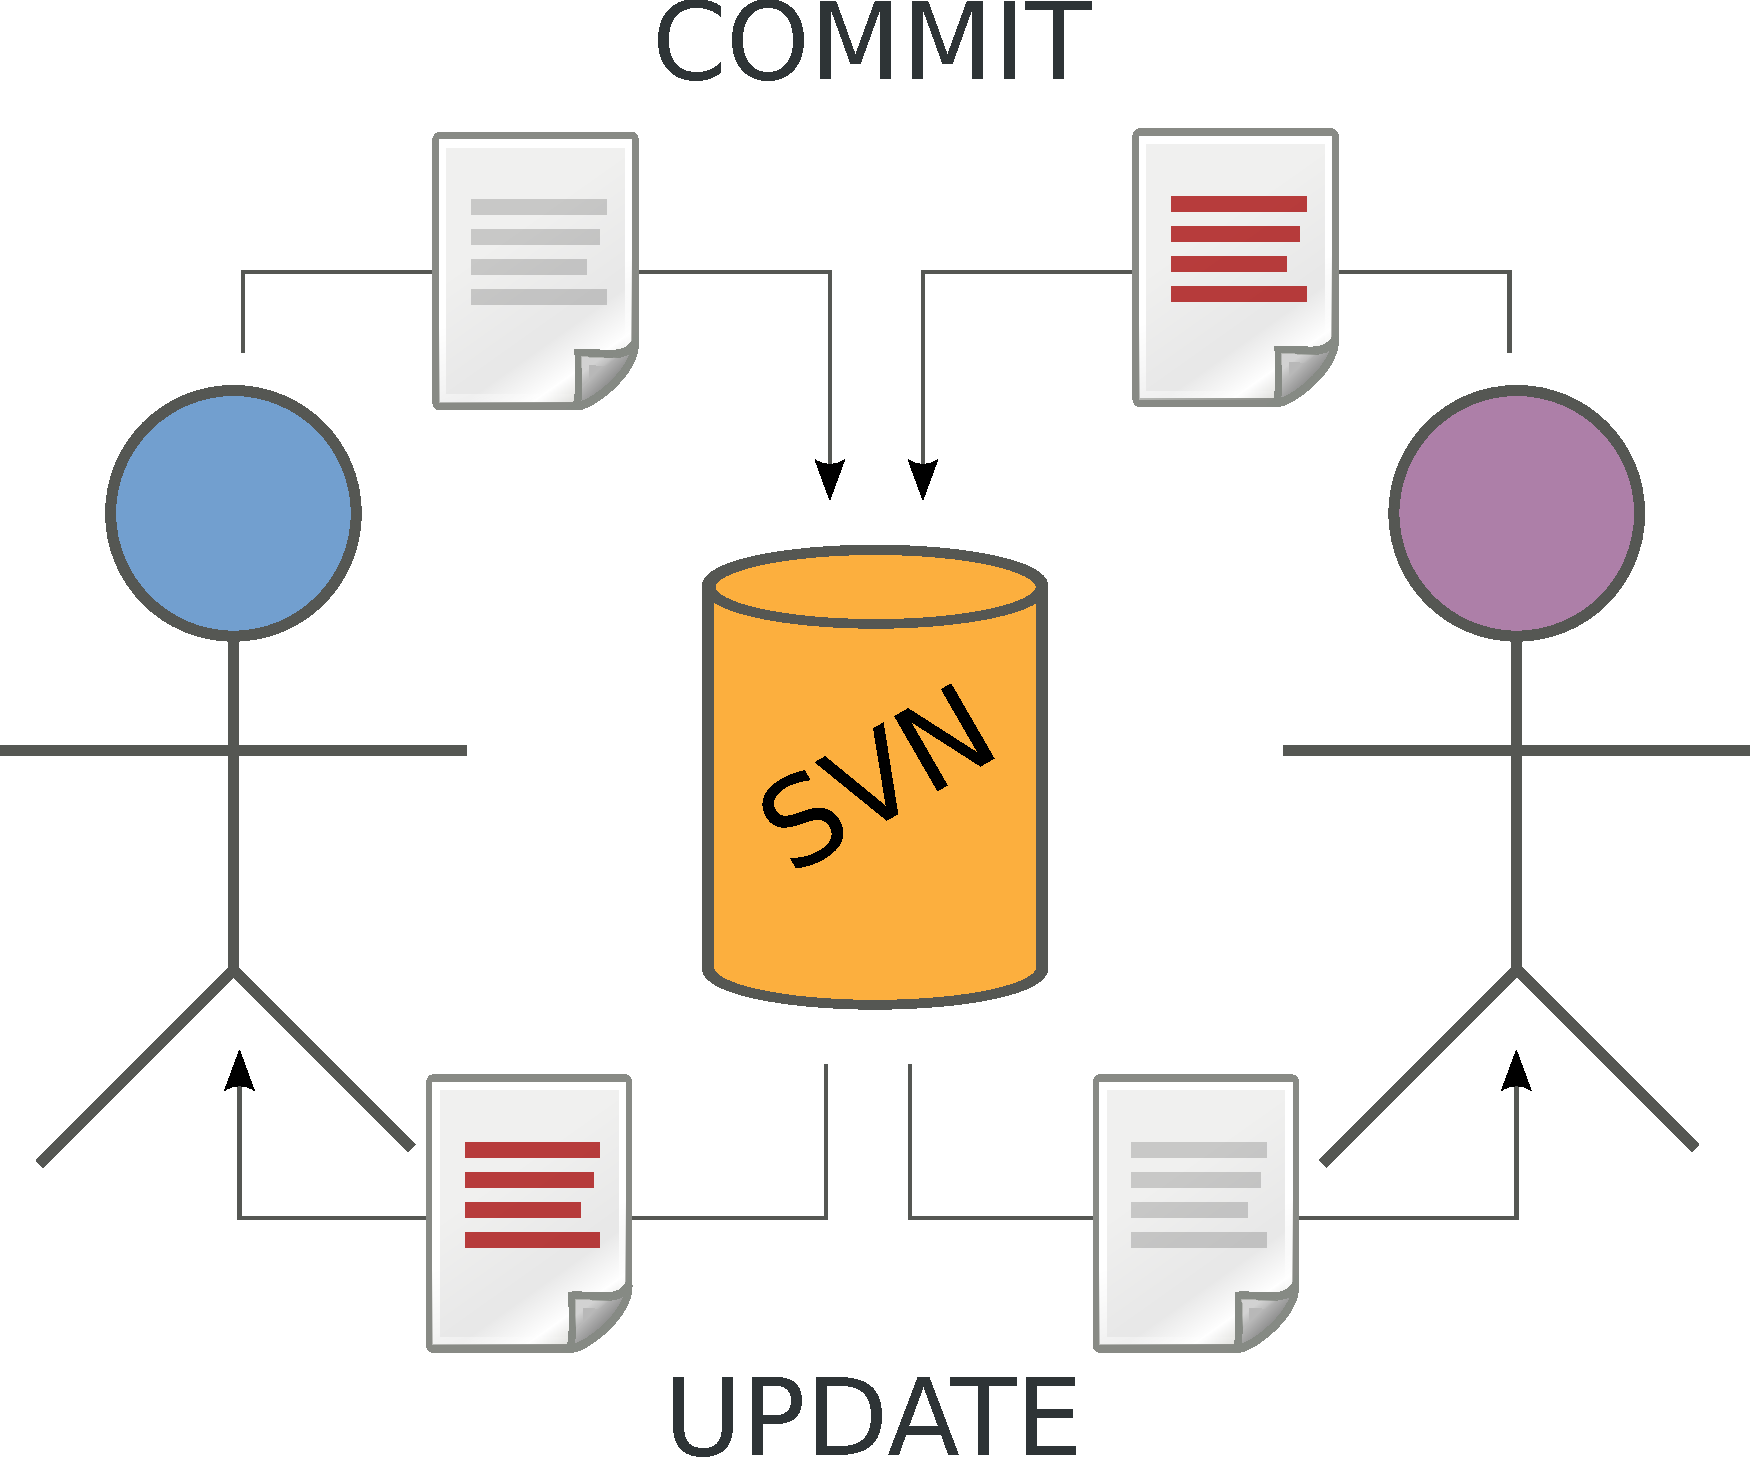
\includegraphics[width=.9\textwidth]{includes/svn.pdf}
    \caption{Solution Subversion}
  \end{figure}
  \end{column}
\end{columns}
\end{frame}

\begin{frame}{Git}
\begin{columns}
  \begin{column}{.55\textwidth}
  Git :
  \begin{itemize}
    \item Logiciel de gestion de versions
    \item Système \textbf{décentralisé} 
  \end{itemize}~

  Pour notre scénario :
  \begin{itemize}
    \item Chaque collaborateur à une copie du PowerPoint (décentralisé)
    \item Les modifications se font en deux temps (différé)
  \end{itemize}
  \end{column}

  \begin{column}{.4\textwidth}
  \begin{figure}
    \center
    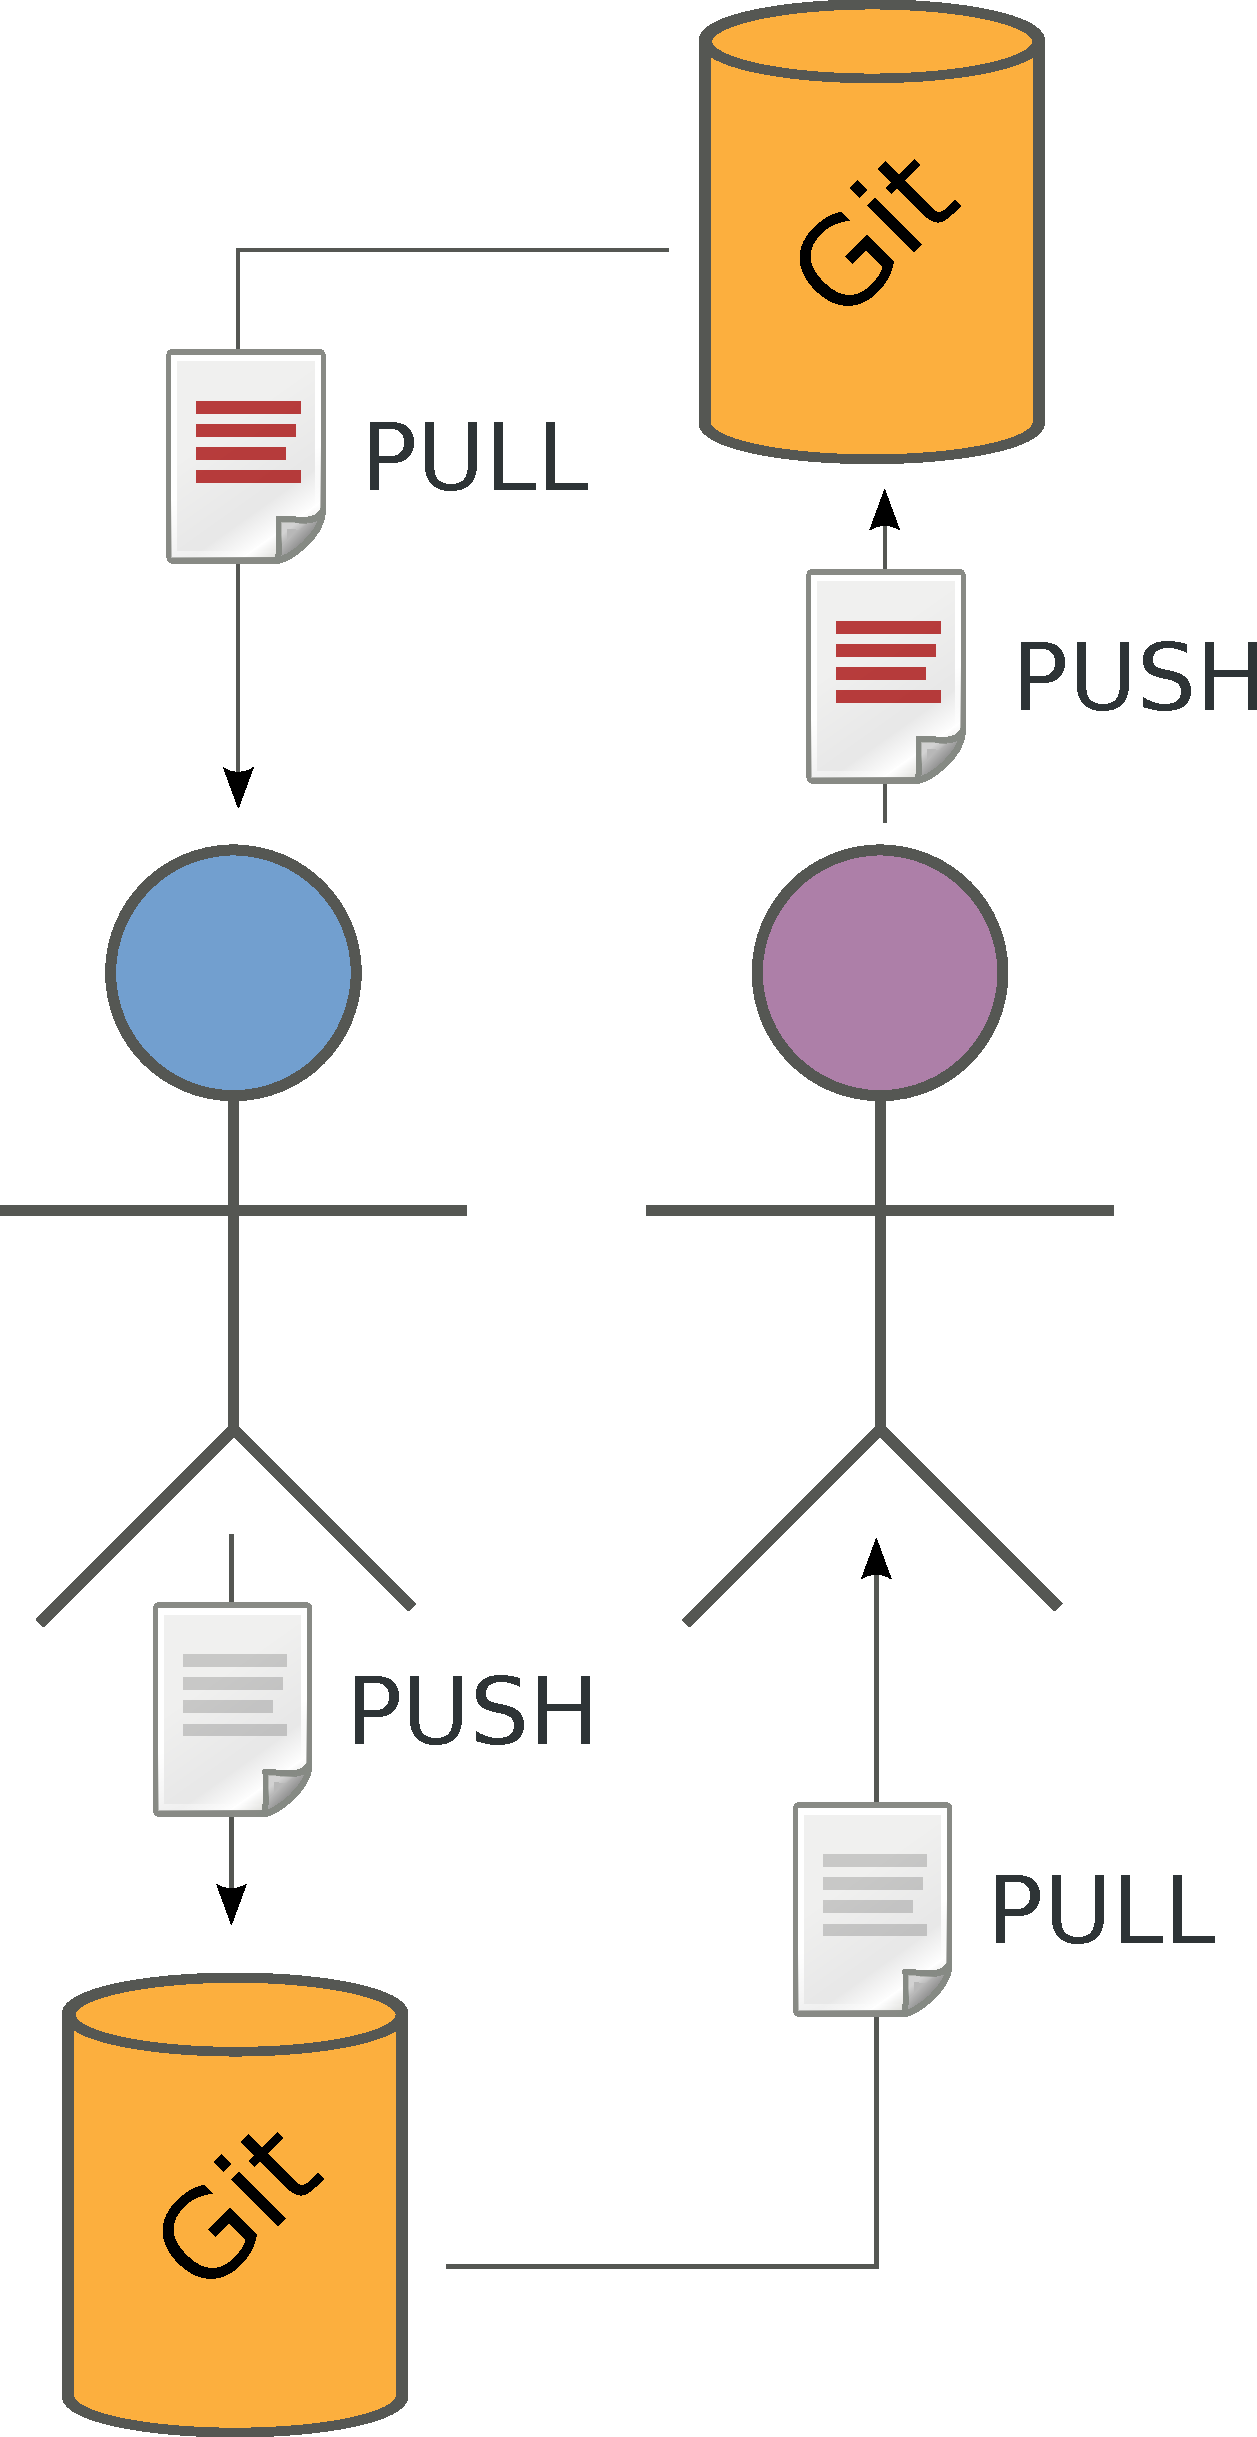
\includegraphics[height=.7\textheight]{includes/git.pdf}
    \caption{Solution Git}
  \end{figure}
  \end{column}
\end{columns}
\end{frame}

\begin{frame}{Google Docs}
\begin{columns}
  \begin{column}{.5\textwidth}
  Google Docs :
  \begin{itemize}
    \item Plateforme pour le travail en ligne collaboratif
    \item Permet l'édition de document Word, Excel et PowerPoint
  \end{itemize}~

  Pour notre scénario :
  \begin{itemize}
    \item Le PowerPoint est sur un serveur (centralisé)
    \item Les modifications se font en instantanées (temps réel)
  \end{itemize}
  \end{column}

  \begin{column}{.45\textwidth}
  \begin{figure}
    \center
    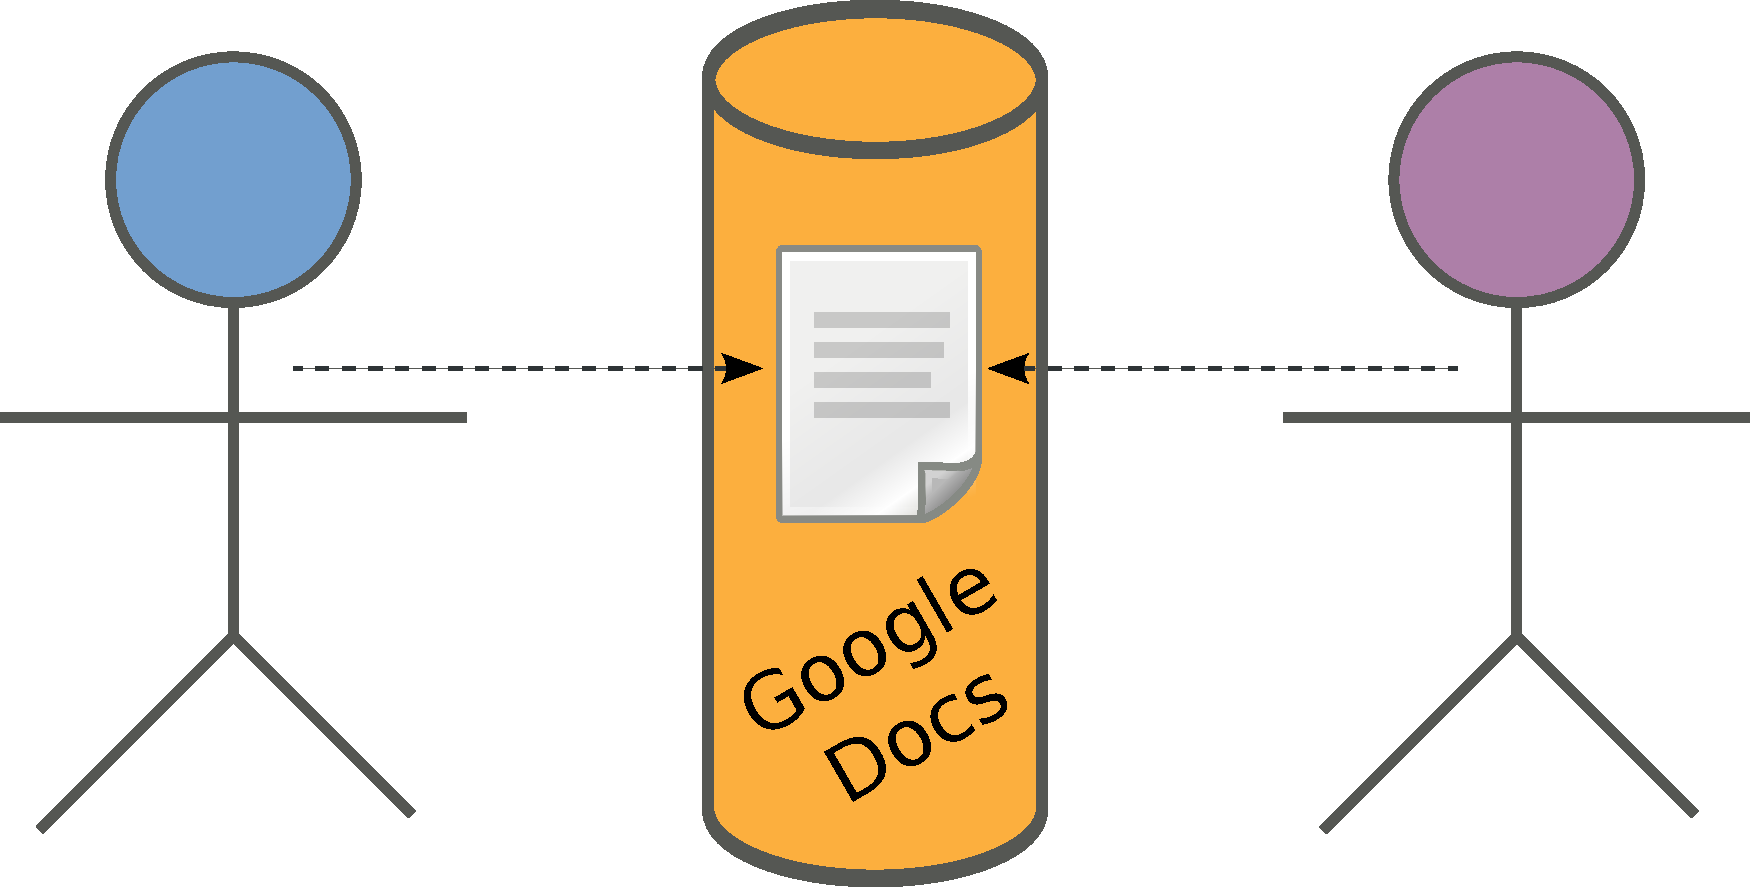
\includegraphics[width=.9\textwidth]{includes/gdocs.pdf}
    \caption{Solution Google Docs}
  \end{figure}
  \end{column}
\end{columns}
\end{frame}

\begin{frame}{Objectifs}
%  \begin{description}
%    \item [Svn] : Document centralisé, Collaboration différée 
%    \item [Git] : Document décentralisé, Collaboration différée
%    \item [Google Docs] : Document centralisé, Collaboration temps réel
%    \item<2-> [CEK-P2P] : \alert{Document décentralisé, Collaboration temps
%    réel}
%  \end{description}
\end{frame}

\begin{frame}{Objectifs}
Un noyau ?
\begin{itemize}
  \item Édition de plusieurs formats de documents : PowerPoint, Code, Partition
  Musicale \ldots 
  \begin{itemize}
    \item Noyau avec un Méta-modèle de document
    \item Utiliser le noyau et se concentrer sur la définition de la structure
    de documents textuels, sans se préoccuper de la distribution des
    modifications dans le réseau
  \end{itemize}
  \item Utiliser le réseau P2P
  \begin{itemize}
    \item Pour transmettre les modifications (medium principal) 
    \item Pour permettre l'envoie de message (exemple : profiter du réseau pour
    proposer un service de chat) 
  \end{itemize}
\end{itemize}
\end{frame}

